% !TEX program = xelatex
% DINOv2 arXiv 2304.07193v2 / TMLR 01/2024, Sections 3-7, Appendix A-B.
% Original imagegen draft retained unchanged via graphicx viewports.
% All math, Chinese labels, arrows and grouping redrawn precisely in TikZ.
\documentclass[tikz,border=2mm]{standalone}
\usepackage{fontspec,xeCJK,amsmath,amssymb,graphicx,lmodern}
\setsansfont{Arial}
\setCJKmainfont[Path=/System/Library/Fonts/,BoldFont={STHeiti Medium.ttc}]{STHeiti Light.ttc}
\setCJKsansfont[Path=/System/Library/Fonts/,BoldFont={STHeiti Medium.ttc}]{STHeiti Light.ttc}
\renewcommand{\familydefault}{\sfdefault}
\usetikzlibrary{arrows.meta,calc}
\definecolor{ink}{HTML}{172D40}
\definecolor{muted}{HTML}{536879}
\definecolor{warm}{HTML}{BA632C}
\definecolor{warmbg}{HTML}{FFF8F0}
\definecolor{teal}{HTML}{087E87}
\definecolor{tealbg}{HTML}{F0FAFA}
\definecolor{blue}{HTML}{2E79A6}
\definecolor{bluebg}{HTML}{F0F7FC}
\tikzset{txt/.style={text=ink,font=\fontsize{16}{20}\selectfont,align=center,inner sep=1pt},
 sm/.style={txt,font=\fontsize{13}{17}\selectfont},
 hd/.style={txt,font=\bfseries\fontsize{21}{25}\selectfont},
 ar/.style={-{Stealth[length=2.2mm]},draw=ink,line width=1.2pt,rounded corners=3pt},
 sup/.style={ar,draw=warm,dashed},
 box/.style={rounded corners=5pt,line width=.8pt,draw=teal!55,fill=white}}
\newcommand{\textat}[4]{\node[txt,text width=#3*.3mm]at(#1,#2){#4};}
\newcommand{\smallat}[4]{\node[sm,text width=#3*.3mm]at(#1,#2){#4};}
\newcommand{\headat}[4]{\node[hd,text width=#3*.3mm]at(#1,#2){#4};}
% Original image is 1024 x 1536 pixels, natural PDF size 1024 x 1536 bp.
\newcommand{\art}[7]{\begingroup
 \pgfmathsetmacro{\bt}{1536-#2-#4}\pgfmathsetmacro{\rt}{1024-#1-#3}
 \pgfmathsetlengthmacro{\aw}{#7*.3mm}
 \node[anchor=north west,inner sep=0,outer sep=0]at(#5,#6){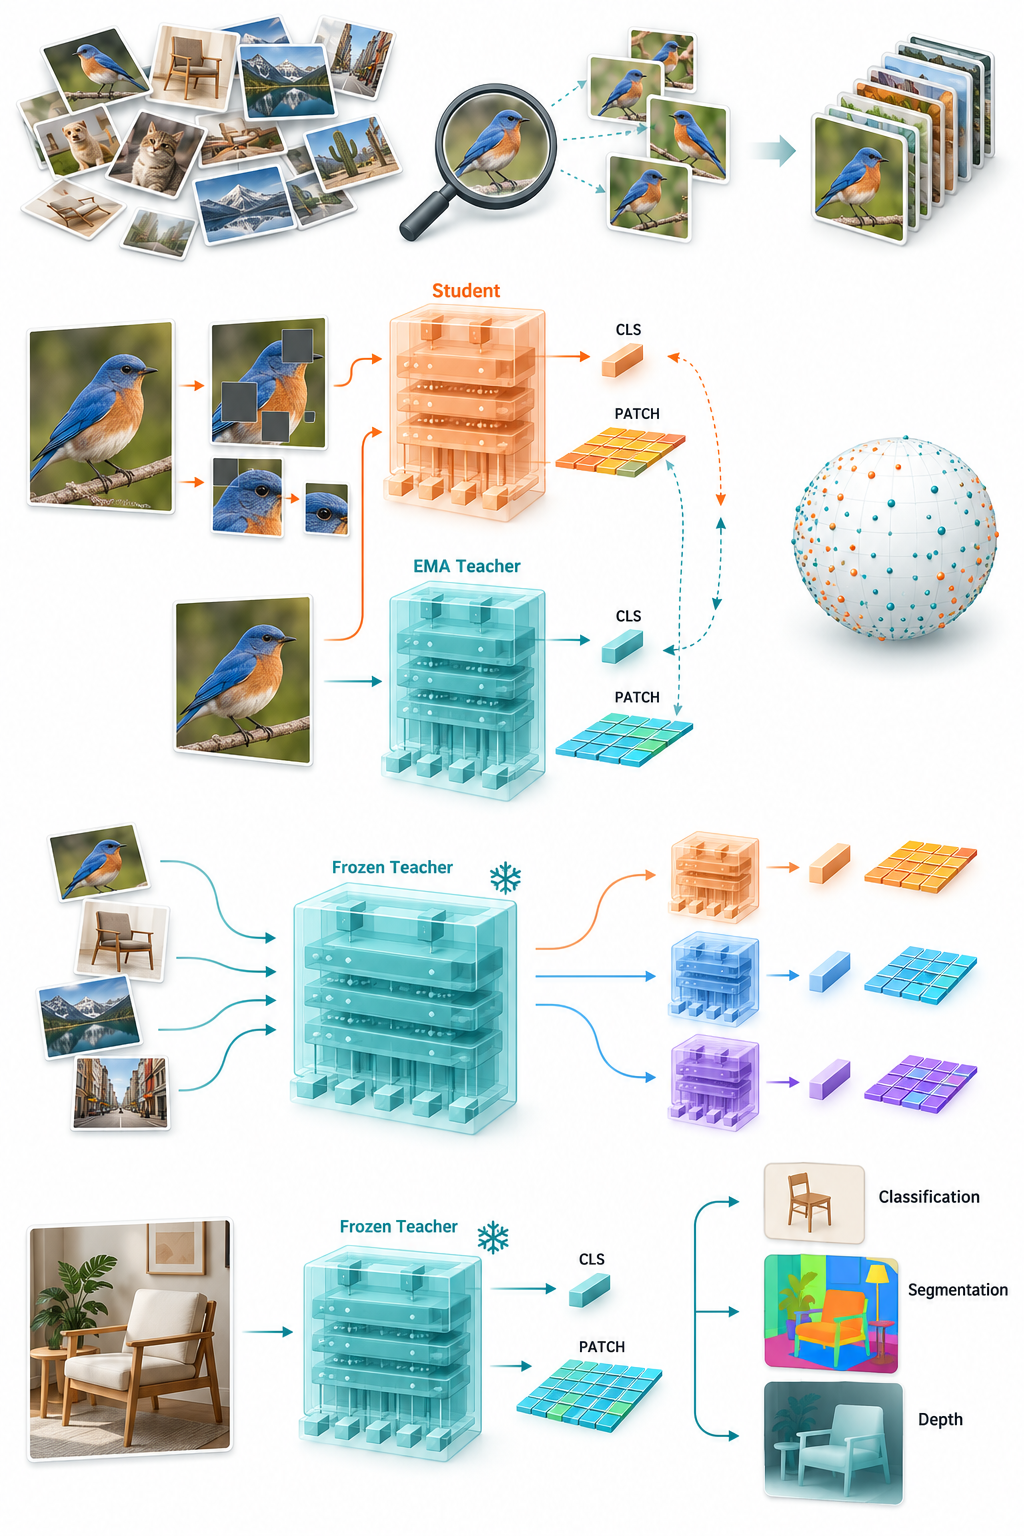
\includegraphics[trim=#1bp \bt bp \rt bp #2bp,clip,width=\aw]{dinov2-imagegen-draft.png}};
\endgroup}
\begin{document}
\begin{tikzpicture}[x=.3mm,y=-.3mm]
\path[use as bounding box](0,0)rectangle(420,1510);
\fill[white](0,0)rectangle(420,1510);
\headat{210}{34}{400}{D\quad 冻结后，特征怎么用？}
\smallat{210}{78}{398}{骨干权重固定；任务头用任务标注训练}
\draw[box,fill=bluebg](8,106)rectangle(412,627);
\art{26}{1225}{209}{238}{37}{143}{115}
\art{301}{1254}{185}{211}{269}{143}{115}
\draw[ar](161,208)--(253,208);
\textat{95}{300}{160}{输入图像 $I$}
\textat{326}{300}{160}{冻结编码器}
\draw[ar](326,327)--(326,363)--(210,363)--(210,387);
\draw[ar](326,363)--(402,363)--(402,512)--(394,512);
\draw[box,draw=blue](31,395)rectangle(389,462);
\textat{210}{428}{348}{全局 CLS：$z\in\mathbb R^d$}
\draw[box,draw=blue](31,479)rectangle(389,546);
\textat{210}{512}{348}{局部 patch：$f_1,\ldots,f_N\in\mathbb R^d$}
\smallat{210}{586}{384}{$224\times224$ 图、$14\times14$ patch\\$N=16^2=256$；ViT-g 的 $d=1536$}

\draw[box,fill=tealbg](8,644)rectangle(412,948);
\headat{210}{679}{385}{1. 全局特征：分类与检索}
\textat{210}{731}{382}{$z\in\mathbb R^d\ \xrightarrow{W,b}\ \ell\in\mathbb R^C$}
\textat{210}{778}{382}{$\ell=Wz+b,\quad p=\operatorname{softmax}(\ell)$}
\smallat{210}{823}{384}{$W\in\mathbb R^{C\times d}$；只训练 $W,b$\\$C$ 是当前分类任务的类别数}
\draw[teal!35,line width=.6pt](32,864)--(388,864);
\textat{210}{902}{380}{图像检索：直接比较特征相似度\\可以不额外训练分类头}

\draw[box,fill=bluebg](8,965)rectangle(412,1455);
\headat{210}{1000}{385}{2. 局部特征：分割与深度}
\textat{210}{1054}{384}{分割：每个 patch 预测类别分数}
\textat{210}{1104}{382}{$N\times d\ \longrightarrow\ N\times C$}
\smallat{210}{1144}{380}{把低分辨率分数图上采样到像素网格}
\draw[blue!35,line width=.6pt](32,1185)--(388,1185);
\textat{210}{1231}{382}{线性深度：每个 patch 拼接 CLS}
\textat{210}{1282}{382}{$[f_i;z]\in\mathbb R^{2d}$}
\smallat{210}{1329}{384}{特征网格双线性上采样 4 倍\\训练深度头，预测 256 个深度区间}
\smallat{210}{1403}{382}{更强的多层读出 / DPT 另有评估协议\\这些任务头不是自监督训练时的 DINO / iBOT 头}
\smallat{210}{1491}{400}{上方 224 像素是形状教学例；各任务评估分辨率见正文}
\end{tikzpicture}
\end{document}
